% Template for PLoS
% Version 2.0 July 2014
%
% To compile to pdf, run:
% latex plos.template
% bibtex plos.template
% latex plos.template
% latex plos.template
% dvipdf plos.template
%
% % % % % % % % % % % % % % % % % % % % % %
%
% -- IMPORTANT NOTE
%
% Be advised that this is merely a template 
% designed to facilitate accurate translation of manuscript content 
% into our production files. 
%
% This template contains extensive comments intended 
% to minimize problems and delays during our production 
% process. Please follow the template 
% whenever possible.
%
% % % % % % % % % % % % % % % % % % % % % % % 
%
% Once your paper is accepted for publication and enters production, 
% PLEASE REMOVE ALL TRACKED CHANGES in this file and leave only
% the final text of your manuscript.
%
% DO NOT ADD EXTRA PACKAGES TO THIS TEMPLATE unless absolutely necessary.
% Packages included in this template are intentionally
% limited and basic in order to reduce the possibility
% of issues during our production process.
%
% % % % % % % % % % % % % % % % % % % % % % %
%
% -- FIGURES AND TABLES
%
% DO NOT INCLUDE GRAPHICS IN YOUR MANUSCRIPT
% - Figures should be uploaded separately from your manuscript file. 
% - Figures generated using LaTeX should be extracted and removed from the PDF before submission. 
% - Figures containing multiple panels/subfigures must be combined into one image file before submission.
% See http://www.plosone.org/static/figureGuidelines for PLOS figure guidelines.
%
% Tables should be cell-based and may not contain:
% - tabs/spacing/line breaks within cells to alter layout
% - vertically-merged cells (no tabular environments within tabular environments, do not use \multirow)
% - colors, shading, or graphic objects
% See http://www.plosone.org/static/figureGuidelines#tables for table guidelines.
%
% For sideways tables, use the {rotating} package and use \begin{sidewaystable} instead of \begin{table} in the appropriate section. PLOS guidelines do not accomodate sideways figures.
%
% % % % % % % % % % % % % % % % % % % % % % % %
%
% -- EQUATIONS, MATH SYMBOLS, SUBSCRIPTS, AND SUPERSCRIPTS
%
% IMPORTANT
% Below are a few tips to help format your equations and other special characters according to our specifications. For more tips to help reduce the possibility of formatting errors during conversion, please see our LaTeX guidelines at http://www.plosone.org/static/latexGuidelines
%
% Please be sure to include all portions of an equation in the math environment, and for any superscripts or subscripts also include the base number/text. For example, use $mathrm{mm}^2$ instead of mm$^2$ (do not use \textsuperscript command).
%
% DO NOT USE the \rm command to render mathmode characters in roman font, instead use $\mathrm{}$
% For bolding characters in mathmode, please use $\mathbf{}$ 
%
% Please add line breaks to long equations when possible in order to fit our 2-column layout. 
%
% For inline equations, please do not include punctuation within the math environment unless this is part of the equation.
%
% For spaces within the math environment please use the \; or \: commands, even within \text{} (do not use smaller spacing as this does not convert well).
%
%
% % % % % % % % % % % % % % % % % % % % % % % %

\documentclass[10pt]{article}
\usepackage{todonotes}
\usepackage{subfigure}
% amsmath package, useful for mathematical formulas
\usepackage{amsmath}
% amssymb package, useful for mathematical symbols
\usepackage{amssymb}
% cite package, to clean up citations in the main text. Do not remove.
\usepackage{cite}
\usepackage{hyperref}
% line numbers
\usepackage{lineno}
% ligatures disabled
\usepackage{microtype}
\DisableLigatures[f]{encoding = *, family = * }
% rotating package for sideways tables
%\usepackage{rotating}
% If you wish to include algorithms, please use one of the packages below. Also, please see the algorithm section of our LaTeX guidelines (http://www.plosone.org/static/latexGuidelines) for important information about required formatting.
%\usepackage{algorithmic}
%\usepackage{algorithmicx}
% Use doublespacing - comment out for single spacing
%\usepackage{setspace} 
%\doublespacing
% Text layout
\topmargin 0.0cm
\oddsidemargin 0.5cm
\evensidemargin 0.5cm
\textwidth 16cm 
\textheight 21cm
% Bold the 'Figure #' in the caption and separate it with a period
% Captions will be left justified
\usepackage[labelfont=bf,labelsep=period,justification=raggedright]{caption}
% Use the PLoS provided BiBTeX style
\bibliographystyle{plos2009}
% Remove brackets from numbering in List of References
\makeatletter
\renewcommand{\@biblabel}[1]{\quad#1.}
\makeatother

% Our defs 
\def \rr {$R_{t}\:$}

% Leave date blank
\date{}

\pagestyle{myheadings}

%% Include all macros below. Please limit the use of macros.

%% END MACROS SECTION


\begin{document}


% Title must be 150 characters or less
\begin{flushleft}
{\Large
\textbf{Estimating the Attack ratio of Dengue Epidemics, under time-varying 
force of infection, from aggregated case notification data}
}
% Insert Author names, affiliations and corresponding author email.
\\
Flavio Code\c{c}o Coelho$^{1\ast}$, 
Luiz Max de Carvalho$^{2}$, 
\\
\bf{1} Escola de Matem\'atica Aplicada , Funda\c{c}\~ao Getulio Vargas (FGV), 
Rio de Janeiro -- RJ, Brazil.
\\
\bf{2} Programa de Computa\c{c}\~ao Cient\'ifica (PROCC), Funda\c{c}\~ao Oswaldo Cruz, Rio de Janeiro -- RJ, Brazil.
\\
$\ast$ E-mail: fccoelho@fgv.br
\end{flushleft}

% Please keep the abstract between 250 and 300 words
\section*{Abstract}
Our paper is just awesome.
% Please keep the Author Summary between 150 and 200 words
% Use first person. PLOS ONE authors please skip this step. 
% Author Summary not valid for PLOS ONE submissions.   
\section*{Author Summary}

\section*{Introduction}

Dengue is a disease which is caused by 4 different types of viruses 
which co-circulate between the vector and human populations. Immunity is 
considered permanent after the exposure of humans to each of the viruses and 
cross immunity is considered very limited\cite{halstead_dengue_2007}.
Thus, the proportions of viral types co-circulating at any point in time is 
strongly dependent on previous incidence of the disease, which determines the 
number of susceptibles for each viral type at any point in time.

Dengue transmission is modulated by environmental conditions, of which 
temperature, due to its effects on the 
vector reproduction, stands out as a strong predictor of 
incidence~\cite{honorio_temporal_2009,wu_higher_2009}.
In places with sufficient temperature variation dengue is predominantly a 
summer disease. So it is fair to say that these environmental fluctuations play 
a key role in determining beginning and end of epidemic periods through its 
effects on the force of infection, which cannot be taken as 
constant\cite{reiner_time-varying_2014}

The long term dynamics of dengue is also modulated by the alternation of virus 
types in circulation. Demographics also plays a role in replenishing the 
population of susceptibles. 

The Attack ratio of disease is a measure of morbidity defined as the number of 
new cases divided by the population at risk.
For Dengue outbreaks and epidemics this can be difficult to calculated due to 
the lack of information about the population at risk. The population at risk in 
the case of dengue, is the number of susceptibles to the circulating virus 
type(s) before a given epidemic.

The main source of information about Dengue dynamics are the incidence 
time series, which represent all the cases of Dengue reported by health 
professionals with no discrimination of virus types.
Only a very small sample 
of the cases are ever examined to determined the virus type.

In order to calculate the attack ratio, we need to determine the number of 
susceptibles to the circulating virus types right before the epidemic.
Without 
regular virological surveys, it is virtually impossible to determine the 
population at risk.

The attack ratio is also influenced by the reproductive number of the disease 
~\cite{bacaer_final_2009, katriel_attack_2012}.
With Dengue, since transmission 
is affected by environmental conditions as discussed above, the reproductive 
number is also expected to vary with time.

Various challenges exist to assess the attack rate of a dengue epidemic. 
One of 
them is that there are a large number of asymptomatic cases in any epidemic, 
which nevertheless acquire immunity.
It is estimated that for 
every case reported, 10-20 are not seen by health authorities (personnal 
communication).
Thirdly, under-reporting is a serious issue in Brazil. 
Duarte and Fran\c{c}a (2006)~\cite{duarte_data_2006}, estimated 
the sensitivity of dengue reporting for hospitalized patients in 
Belo-Horizonte, Brazil to be of 63\%, 
meaning that approximately 37\% of the suspected dengue cases go unreported.  
Lastly, demography and migrations affect the number of susceptible in ways which 
are not easy to determine.


In this paper, we estimate the number of susceptibles before every major 
outbreak ($S_{0, year}$) in the last 18 years.
Due to the alternation of circulating serotypes, we detected fluctuating levels 
of susceptibility the circulating virus(es).
To estimate the susceptibles we have we have fixed the 
transmissibility based on the $R_t$ series derived from data~\cite{nishiura}. 
Then, 
from the incidence series and the population at risk, we could then calculate 
the attack ratio for each epidemic.

To accomplish the estimation of the $S_0$, we use a simplified model of 
dengue transmission based on a single-strain Susceptible-Infecctious-Removed 
(SIR) model.
The reason for the choice of a single strain model, is the lack of 
accurate information regarding the actual proportions of each virus in 
circulation.
However, some information is available about the predominant 
serotypes for some epidemics in the period 
of study~\cite{macedo_virological_2013}. 

Methods for estimating the  number of susceptibles have been proposed 
before, for other diseases~\cite{bjornstad_dynamics_2002, 
wallinga_reconstruction_2003}.
These methods try to reconstruct the entire 
series of infectious and susceptibles for measles 
outbreaks from case data.
In the case of Dengue, the full (multi-year/multi-epidemic)
series of susceptibles to all possible serotypes, cannot be reconstructed based 
solely on a deterministic transmission model, since the arrival/re-emergenge of 
new serotypes (which are a stochastic events) can change drastically the pool 
of susceptibles throwing off any sequential estimation based on the incidence
dynamics.

The authors have applied similar methods as used here, to estimate the number 
of susceptibles for the predominant strain of Influenza at the beginning of  
Influenza seasons in europe~\cite{pone2011}.


\section*{Methods}



In this section we will start by describing the data and then the method used 
to estimate the effective reproductive number, $R_t$, from the data and obtain 
its posterior distribution. 
We then proceed to describe Susceptible-infectious-recovered (SIR) model 
used to represent the global disease incidence and how $R_t$ can be integrated 
into the model to allow for time varying transmission. 
Next, an approach to approximate the posterior distributions 
of the numbers of susceptible to the main circulating Dengue viruses for each 
epidemic is detailed.
Finally, we discuss how to estimate the attack ratio of each 
epidemic using the estimated susceptible fraction and observed incidence.


\subsection{The dataset} 
The data used in this paper consists of  Dengue weekly notified cases time 
series for the city of Rio de Janeiro from 1996 to 2014. The cases are notified 
based only on clinical symptoms. Laboratory confirmation and serotype 
information are available only for a very small sample and only on recent 
years (2010-2013). The incidence is normalized for the parameter estimation 
procedures. The normalizatio was done by dividing the number os cases reported 
by the total city population at each year as given by the census.

\subsection*{Estimating the effective reproductive number ($R_t$)}

In monitoring of infectious diseases, it is important to assess whether the 
incidence of a  particular disease is increasing significantly, in order to 
decide to take preventive measures.
The effective reproductive number at time $t$, \rr, can be understood as a 
real-time estimate of the basic reproductive number ($R_{0}$) and is defined as 
the average number of secondary cases per primary case at time $t$.

Let $Y_t$ be the number of reported disease cases for a particular time $t \in 
(0, T)$.
Nishiura el al. (2010)~\cite{nishiura} extend the theory developed by 
Stallybrass et al. (1931)~\cite{stallybrass} and propose to estimate \rr as
\begin{equation}
\label{eq:Rtestimate}
R_t = \left( \frac{Y_{t+1}}{Y_t}\right)^{1/n}
\end{equation}
where $n$ is taken to be the ratio between the length of reporting interval and 
the mean generation time of the disease.
Here we are interested in the simpler case $n=1$.
If \rr is to be used as a decision tool, however, one needs to be able to 
quantify the 
uncertainty about estimate in equation~\ref{eq:Rtestimate}. 
Here we detail how to obtain credibility intervals for \rr under the assumption 
that the counts $Y_t$ are Poisson distributed for all $t$.

We explore the approach of Ederer and Mantel~\cite{mantel}, whose objective is 
to obtain 
confidence intervals for the ratio of two Poisson counts. 
Let $Y_{t} \sim Poisson(\lambda_t)$ and $Y_{t+1} \sim Poisson(\lambda_{t+1})$ 
and define $S = Y_{t} + Y_{t+1}$.
The authors note that by conditioning on the sum $S$
\begin{align}
\label{eq:binlike}
Y_{t+1} | S &\sim Binomial(S, \theta_t) \\
\theta_t &= \frac{\lambda_{t+1}}{\lambda_{t} + \lambda_{t+1}}
\end{align}
Let $c_{\alpha}(\theta_t) = \{\theta_t^{(L)} , \theta_t^{(U)} \}$ be such that 
$Pr(\theta_t^{(L)}<\theta_t <\theta_t^{(U)}) = \alpha$.
Analogously, define $c_{\alpha}(R_t) = \{R_t^{(L)} , R_t^{(U)} \}$ such that 
$Pr(R_t^{(L)}<R_t<R_t^{(U)}) = \alpha$.
Ederer and Mantel (1974)~\cite{mantel} show that one can construct a $100\alpha 
\%$ confidence interval for \rr by noting that
\begin{align}
\label{eq:confRt}
 R_t^{(L)} &= \frac{\theta_t^{(L)}}{(1-\theta_t^{(L)})}\nonumber \\
 R_t^{(U)} &= \frac{\theta_t^{(U)}}{(1-\theta_t^{(U)})}
\end{align}
Many authors have derived $c_{\alpha}(\theta_t)$ following orthodox approaches  
(see for example~\cite{wilson} and~\cite{clopper}) mainly for simplicity.
We choose instead to take a Bayesian approach and use the  $100\alpha \%$ 
posterior credibility interval for $\theta_t$ as $c_{\alpha}(\theta_t)$.
If we choose the conjugate beta prior with parameters $a_0$ and $b_0$ for the 
binomial likelihood in (\ref{eq:binlike}), the posterior distribution for 
$\theta_t$ is
\begin{equation}
\label{eq:thetapost}
p(\theta_t| Y_{t+1}, S) \sim Beta(Y_{t+1} + a_0, Y_t + b_0)
\end{equation}
Combining equations~(\ref{eq:confRt}) and~(\ref{eq:thetapost}) 
tells us that the induced posterior distribution of $R_t$ is 
a beta prime (or inverted beta) with parameters $ a_1 = Y_{t+1} + a_0$ and $b_1 
=  Y_t + b_0$.
The density of the induced distribution is then 
\begin{equation}
\label{eq:densityMantel}
f_P(R_t| a_1, b_1) = \frac{\Gamma(a_1 + b_1)}{\Gamma(a_1)\Gamma(b_1)} R_t^{a_1 - 
1} (1 + R_t)^{-(a_1 + b_1)}
\end{equation}
Thus, the expectation of \rr is $a_1/(b_1 - 1)$ and its variance is 
$a_1(a_1 + b_1 - 1)/\left((b_1 - 2)(b_1 - 1)^2 \right) $.
Sampling from the posterior in~(\ref{eq:densityMantel}) can be made 
straightforward by first sampling from~(\ref{eq:thetapost}) and then applying 
the transform in~(\ref{eq:confRt}).
Also, one can choose $a_0$ and $b_0$ so as to elicit meaningful prior distributions
for $R_t$.
We show how to elicit the prior for $R_t$ from specified prior mean and variance
or coefficient of variation in Text S1.

Also, since $R_t > 1$ indicates sustained transmission, one may be 
interested in computing the probability of this event.
This can be easily achieved by integrating~(\ref{eq:densityMantel}) over the 
appropriate interval.
By noting that
\begin{align}
\label{cumprobMantel}
Pr(R_t > 1) &= 1 - \int_0^1 f_P(r)dr \\
            &= 1- Pr(\theta_t < \frac{1}{2})
\end{align}
one can compute the desired probability while avoiding dealing with the density 
in~(\ref{eq:densityMantel}) directly.

\subsection*{Mathematical modeling} % The model

A Susceptible-Infectious-Removed (SIR) model is proposed to model dengue 
dynamics.
In the traditional formulation of the model, transmission is governed by a 
constant transmission rate $\beta$ and recovery happens at a rate $\tau$.

For our analysis we chose to let the force of infection vary with time, just 
as it does in the actual epidemics, as seen in the data. So as the epidemic 
progresses, the effective transmission  rate changes and is 
given by 
\begin{equation} 
 \label{eq:effbeta}
 \beta(t) = \frac{R_t\cdot\tau}{S_0}
\end{equation}
where $R_t$ is the effective reproductive number, estimated as 
in~\ref{eq:Rtestimate}.
The complete model with the time-verying force of infection is given by
the system of ordinary differential equations below.
\begin{align}
   \label{eq:model}
 \frac{dS}{dt} &= -\beta(t)SI \\     \nonumber
 \frac{dI}{dt} &= \beta(t)SI - \tau I&\\      \nonumber
 \frac{dR}{dt} &= \tau I&
\end{align}  
where $S + I + R = 1 \: \forall\: t$. % \in [T_0, T_1]$. 
Of course, this is a rather simplified model, in which, for instance, the 
vector is omitted.
The rationale for this simplification is based on the ability of the 
empirically derived $R_t$  to incorporate the effects of the fluctuating vector 
populations.
Also, although there are multiple circulating serotypes, our approach
can not discriminate between them due to the lack of serotype-specific data.
Nevertheless, this modeling strategy can still provide some insight into the 
disease dynamics and allows us to estimate the initial fraction of susceptibles 
$S_0$.

\subsection*{Bayesian parameter estimation}
We take a Bayesian approach to the estimation of $S_0$.
First the incidence time series was divided into $J=13$ 
epidemic windows that corresponded to significant raises in incidence and 
normalized to lie on the $[0,1]$ interval.
For a given interval $j = \{ t_j^{\text{start}}, t_j^{\text{end}} \} $ we 
observe an incidence time series $\mathbf{Y_{j}}$.
We are thus interested in the posterior distribution
\begin{equation}
 \label{eq:S0post}
 p(S_{0j}|\mathbf{Y_{j}}) \propto l(\mathbf{Y_{j}}|S_{0j}, R_t, m, \tau 
)\pi(S_{0j}) 
\end{equation}
The likelihood $l(\mathbf{Y_{j}}|\cdot)$ is assumed to be a Normal distribution 
with fixed variance $\sigma^2$.
In this estimation procedure we kept $R_t$ fixed at fixed at the posterior mean 
obtained as described above and fixed $\tau = 1/7\: \text{days}^{-1}$.
To complete the inference, we need to specify prior distributions for the 
parameters of interest.
We place a flat $\text{Beta}(1, 1)$ prior on $S_{0j}\:\forall j$

To approximate the posterior in~(\ref{eq:S0post}) we use Markov chain Monte 
Carlo techniques implemented in the Bayesian inference with Python 
(BIP)~\cite{pone2011} available at  
\url{http://code.google.com/p/bayesian-inference/}.
BIP uses a Differential Evolution Adaptive Metropolis (DREAM)~\cite{vrugt2008} 
scheme that efficiently samples from high-dimensional joint distributions using 
multiple adaptive chains running in parallel with delayed rejection.
Also, as the numerical integration routine implemented within BIP needs 
$\beta(t)$ to be available at 
arbitrary values of $t$, i.e., as continuous function of time because of the 
variable step size, we used linear interpolation to obtain values of $R_t$ for 
any time point.
In this study we used one chain per parameter, i.e, 3 chains for each run.
The chains were run until $5000$ samples were obtained after discarding $500$ 
burn-in samples.
Convergence of the parallel chains was verified at every 100 iterations by the 
calculation of the Gelman-Rubin's R convergence diagnostic~\cite{brooks1998}.

\subsection*{Calculating the attack ratio}

The attack ratio of an epidemic is define by the number of infections divided 
by the size of the population at risk.

\begin{equation}
\label{eq:AR}
A=\frac{\text{\# cases}}{\text{Population at risk}} 
\end{equation}

Based on what has been discussed so far, we can rewrite (\ref{eq:AR}) for 
each epidemic $j$ as
\begin{equation}
\label{eq:AR2}
 A_{j}=\frac{\sum Y_j}{S_{0j}}
\end{equation}
where $S_{0j}$ is the number of susceptibles before each epidemic $j$, which we
estimated before.

\section*{Results and Discussion}
 
Figure \ref{fig:rtseries}  shows the $R_t$ series, according to 
(\ref{eq:Rtestimate}). 
It can be seen that the inter-epidemic periods are characterized by $R_t$ being 
indistinguishable from 1. Due to the instrinsic variability of the \rr series, 
the exmination of its credible intervals is essential to identify periods 
of sustained transmission. The wider credible intervals for the interepidemic 
periods are due to the scarsity of cases. Our methodology to derive the 
probability distribution for \rr is an original contribution applicable to the 
analysis of any incidence time-series of  any transmissible disease.

\begin{figure}
 \centering
 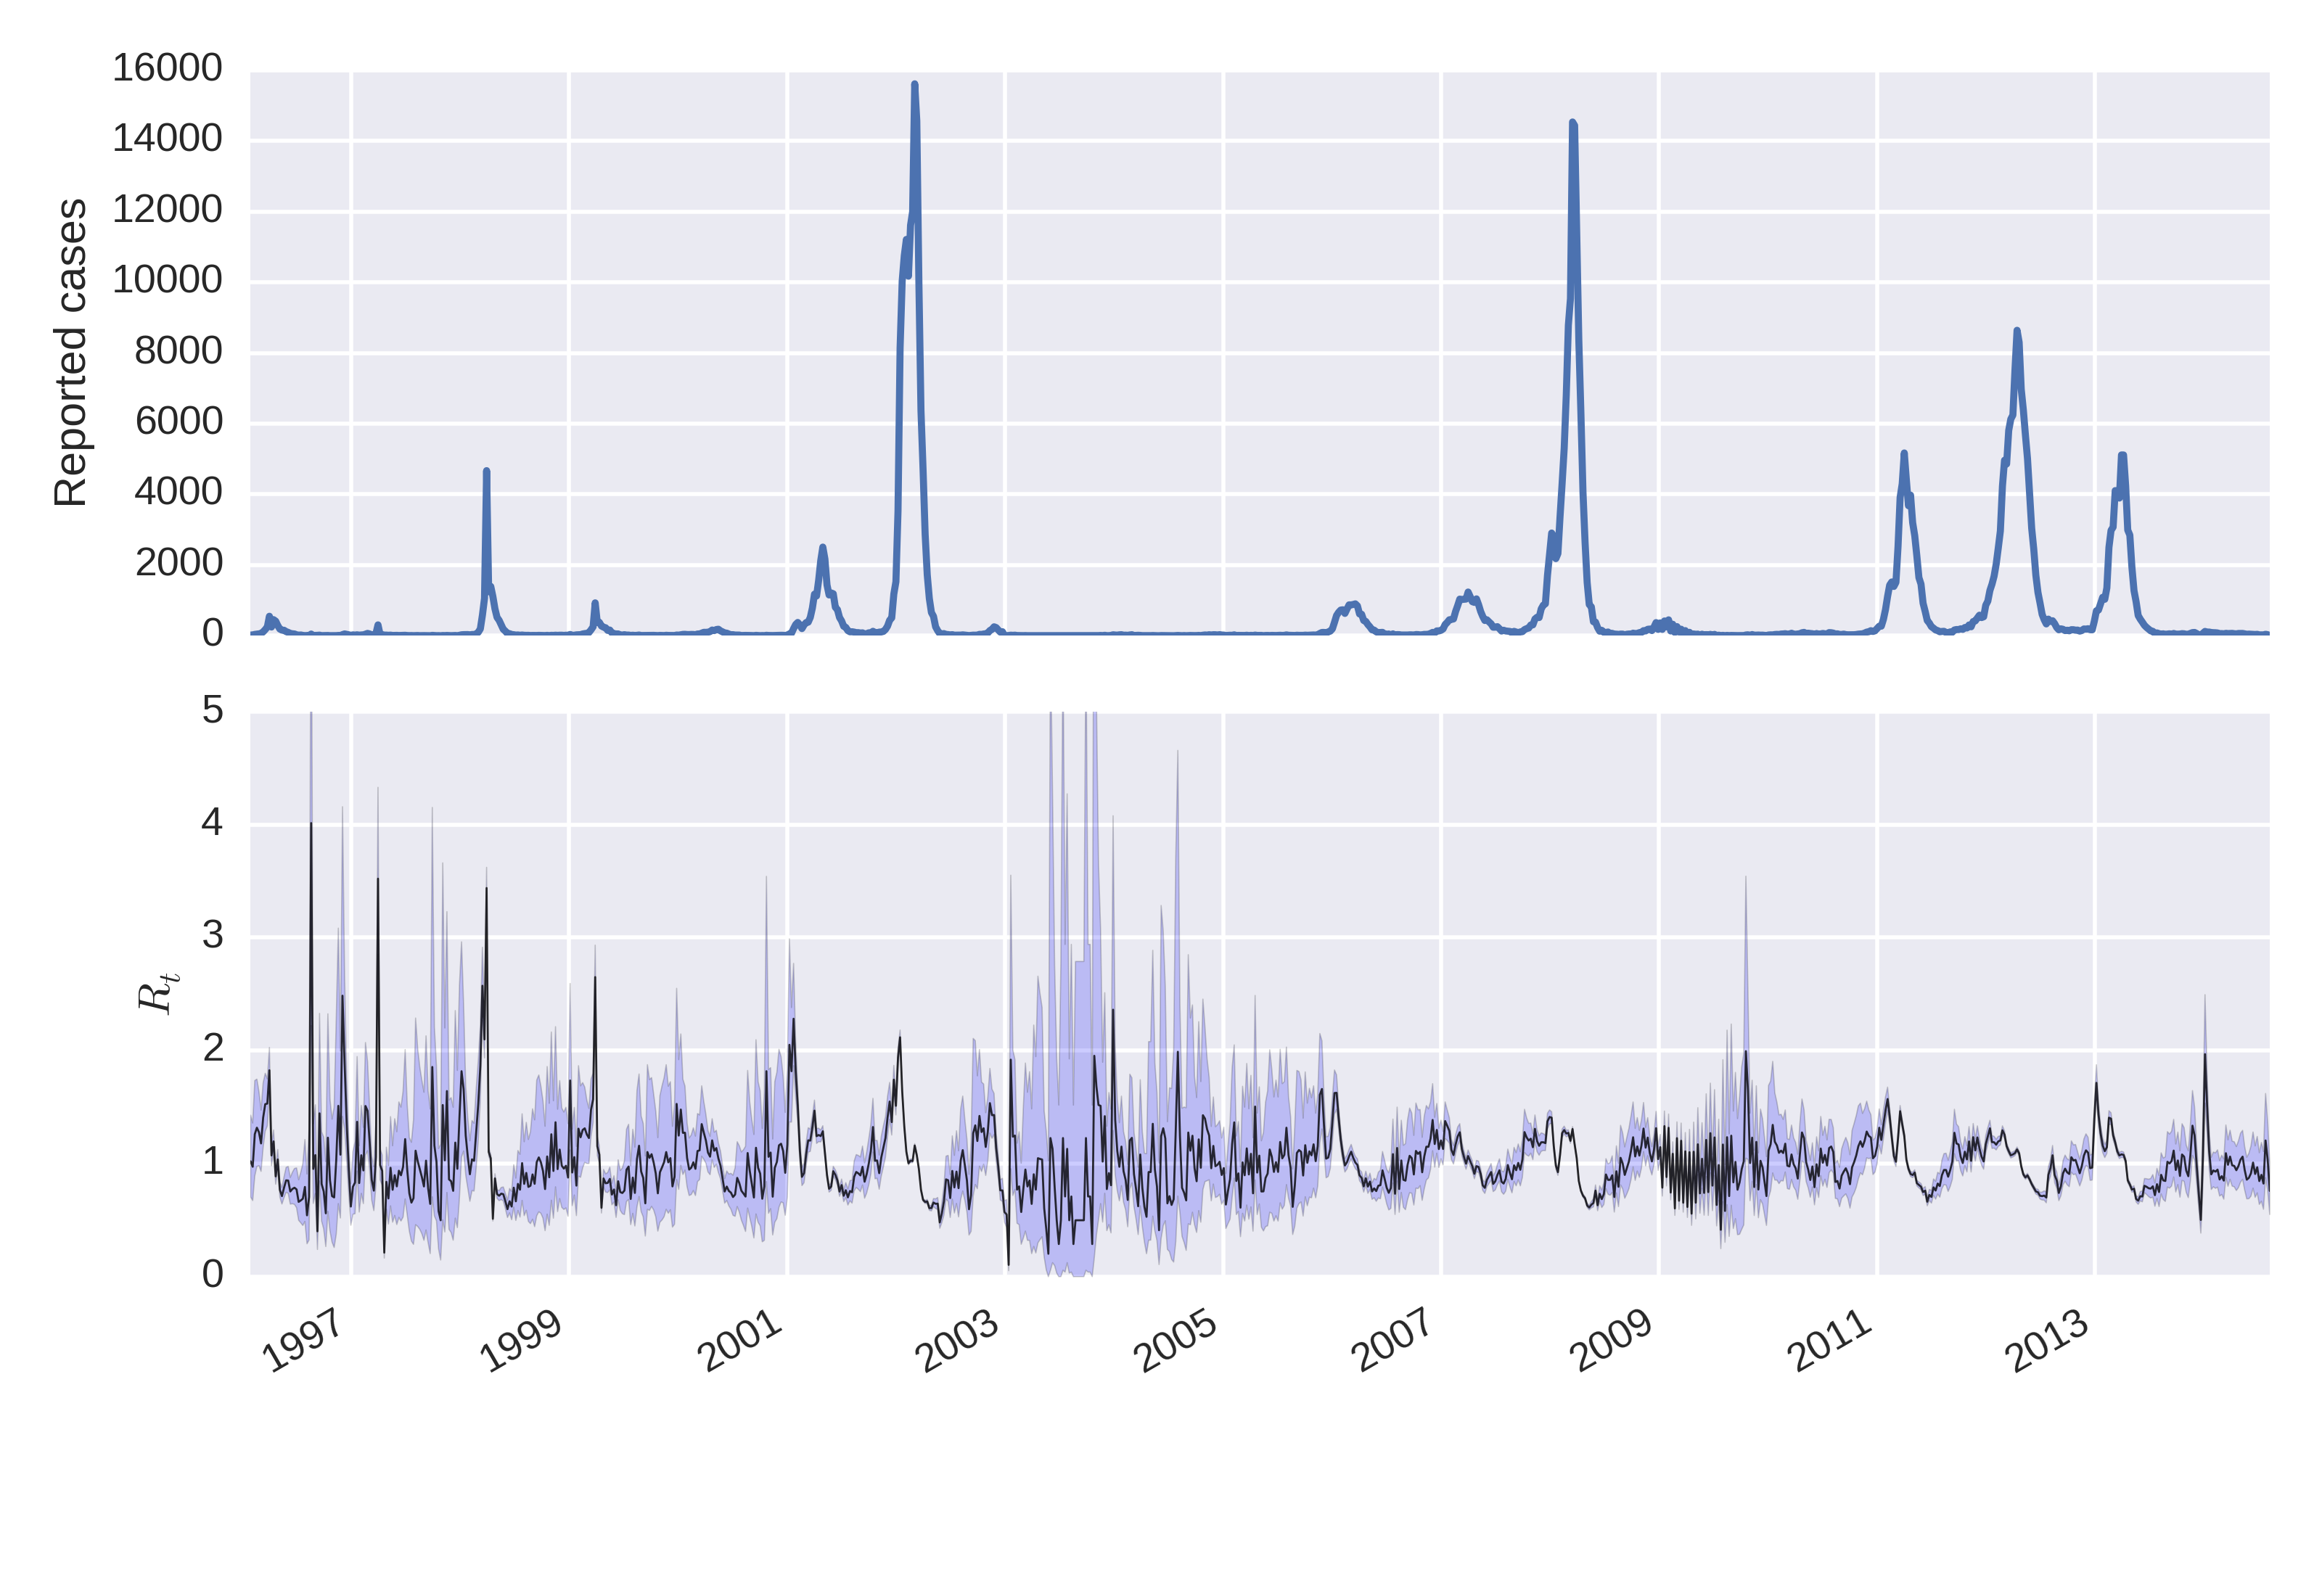
\includegraphics[width=16cm]{./plots/rt_series.png}

 \caption{{\bf Estimated time-series for $R_t$, along with 95\% credible 
intervals.} Top panel show reported cases from which $R_t$ is estimated.}
 \label{fig:rtseries}
\end{figure}


Figure \ref{Fig:S0}, shows the model from (\ref{eq:model}) fitted to the data. 
In it we can see that the susceptibles series in each epidemic starts at the 
estimated level of $S_0$.
The proportion of susceptibles may seem low, but we 
must remember that these estimates are being affected by an unknown 
underreporting factor, which experts suggest is somewhere between 5 and 10, 
i.e. for every case observed there are 5 or 10 unobserved.
Since this underreporting affects both the numerator and denominator of 
(\ref{eq:AR}), its effects should cancel out, giving us an unbiased attack ratio 
estimate.
One other possible source of bias which would lead to the 
underestimation of $S_0$ could come from a significant part of the population 
not being exposed to the disease.
However, as we can see in figure \ref{fig:mapas} , the disease spreads pretty 
much homogeneously over 
the entire city (in the last four epidemics, at least). 

\begin{figure}
 \subfigure[2010]{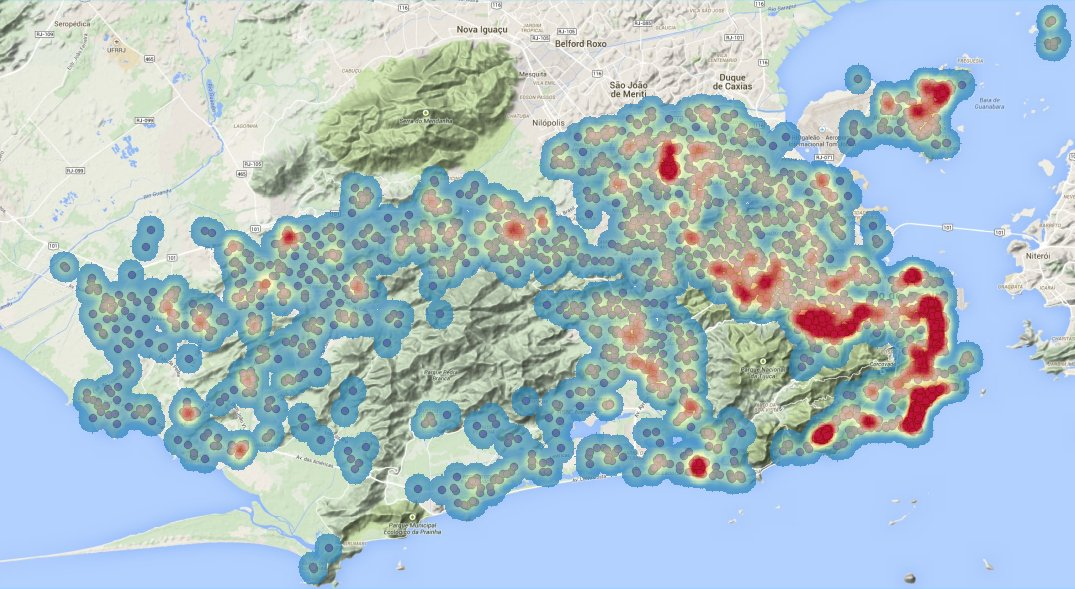
\includegraphics[width=8cm, 
height=4.82cm]{./plots/heatmap2010.jpg}
% heatmap2010.jpg: 1075x589 pixel, 96dpi, 28.44x15.58 cm, bb=0 0 806 442
}
  \subfigure[2011]{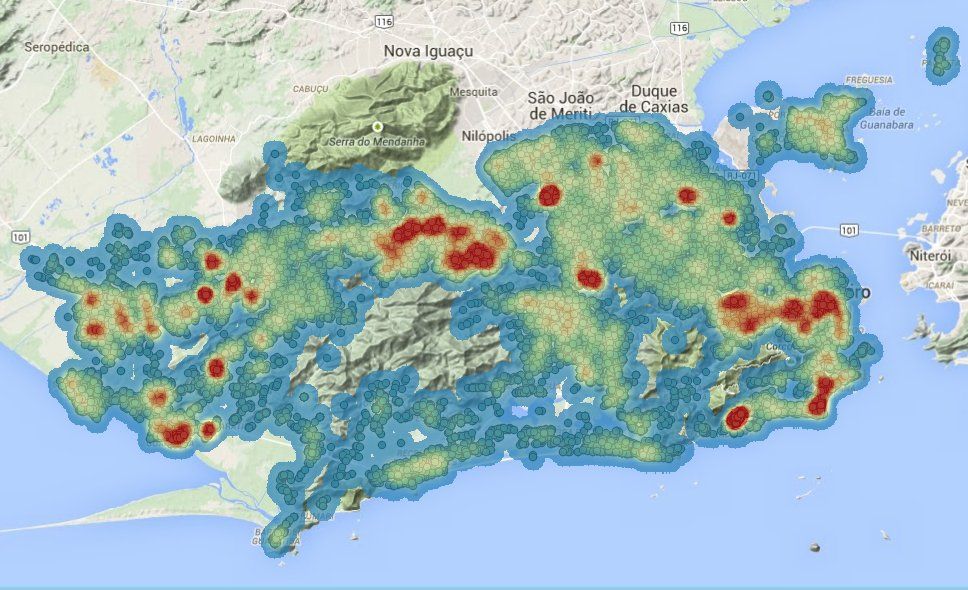
\includegraphics[width=8cm]{./plots/heatmap2011.jpg}}
  \subfigure[2012]{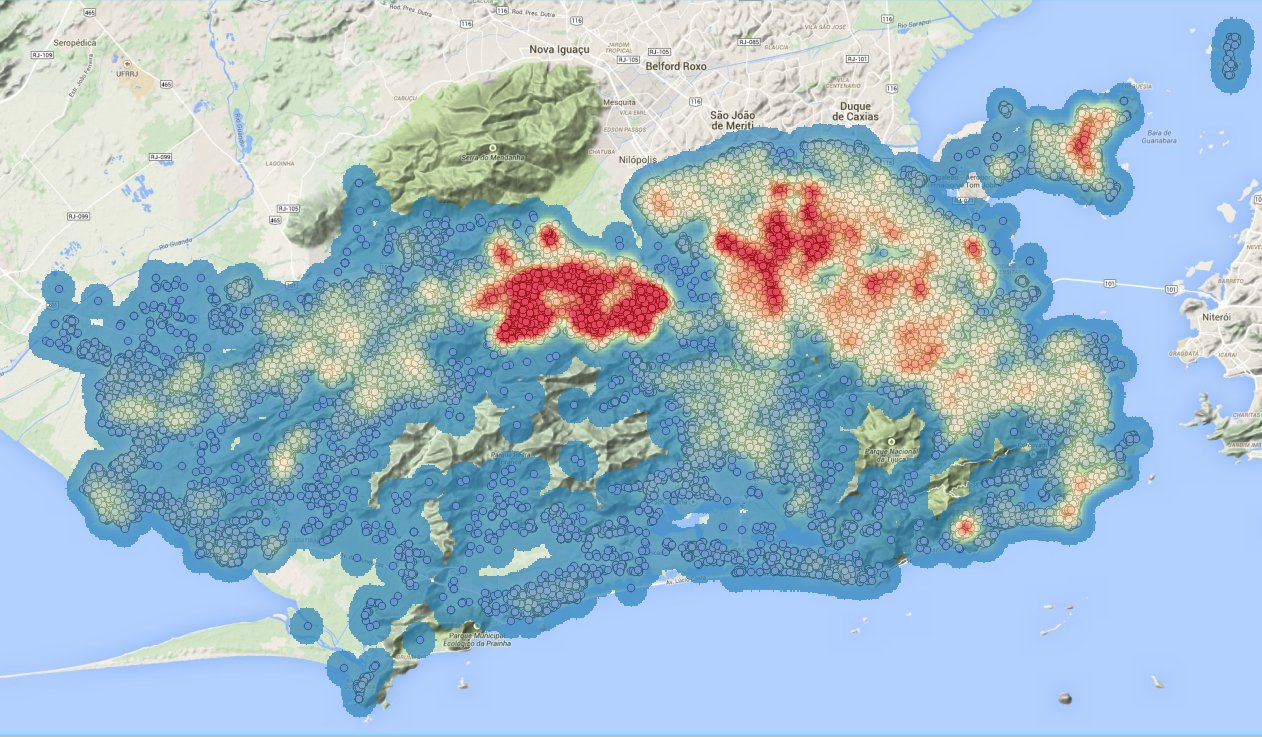
\includegraphics[width=8cm]{./plots/heatmap2012.jpg}
% heatmap2010.jpg: 1075x589 pixel, 96dpi, 28.44x15.58 cm, bb=0 0 806 442
}
  \subfigure[2013]{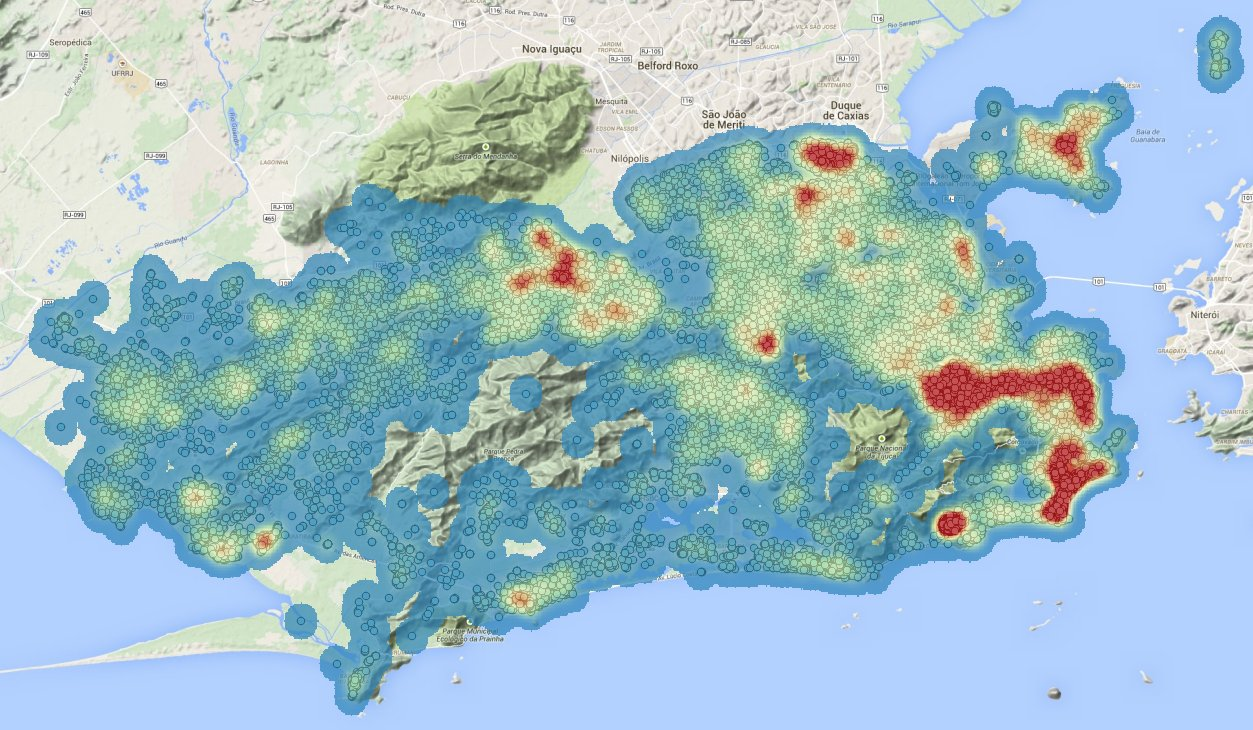
\includegraphics[width=8cm]{./plots/heatmap2013.jpg}}
  \caption{{\bf Maps showing the incidence of dengue in the city of Rio de 
Janeiro from 2010 to 2013.} Circles indicate individual notified cases. A 
heatmap is overlayed on the maps showing absolute density of cases.}
  \label{fig:mapas}
\end{figure}


Table \ref{tab:AR} contains the attack ratios and medians of the $S_0$ 
estimated for each epidemic/outbreak. It is interesting to notice that the 
larger epidemics, in terms of total number of cases are not the one with the 
greater attack ratios. This stresses the importance of knowing the imunological 
structure of the population in order to truly assess the impact of eny 
epidemic. 

The authors hope that this evidence will motivate public health 
outhorities to invest in annual serological surveys, to determine the 
susceptibility profile to each dengue virus as well as to estimate the 
underreporting factor of the notification system.
% We only support three levels of headings, please do not create a heading level below \subsubsection.
%\subsection*{Subsection 1}
%\section*{Discussion}
% Do NOT remove this, even if you are not including acknowledgments.
\section*{Acknowledgments}
LMC is grateful to Dr. Leonardo Bastos for useful discussions on the 
posterior inference for $R(t)$.
The authors are also grateful to Claudia T. 
Code\c{c}o for helpful discussions about the manuscript.

\section*{Appendix}
\subsection*{A remark on prior distributions and tail behavior of the 
distribution of $R_t$}
\label{sec:tails}
There are a number of approaches to deriving the distribution of \rr.
Alternatively to the approach described in the main text\cite{mantel}, one 
could use the conditional distribution of \rr on 
$Y_{t+1}$ and $Y_t$ as defined in equation A7 of Nishiura et al.\cite{nishiura}:
\begin{equation}
\label{seq:unorm}
f_{R}(R_{t}) = (Y_tR_{t})^{Y_{t+1}} e^{-Y_tR_{t}}
\end{equation}
Noticing the kernel of (\ref{seq:unorm}) is that of a gamma distribution with 
$a_2 = Y_{t+1}+1$ and $b_2 = Y_t$, we obtain a proper density from which to 
construct $c_{\alpha}(R_t)$, simply by computing the appropriate quantiles of 
said distribution.
 This density is
\begin{equation}
\label{seq:densityNishiura}
f_N(R_t| a_2, b_2) =  \frac{b_2^{a_2}}{\Gamma(a_2)} R_t^{a_2-1} e^{-b_2 R_t}
\end{equation}

In order to decide which approach to take, it may be of use analyzing the 
variance and tail behavior of the derived distributions for \rr. 
Consider the case of using a flat $Uniform(0, 1)$ prior for $\theta_t$.
With $a_0 = b_0 = 1$, $a_1 = a_2$ and $b_1 = b_2 + 1$.
The beta prime (inverse beta distribution) will have heavier tails compared to 
the conditional distribution proposed by~\cite{nishiura}, thus providing more 
conservative confidence/credibility intervals.
To see that one needs simply take the ratio of the Beta prime and Gamma 
(unnormalized) densities and evaluate the limit as $R_t$ goes to infinity:
\begin{equation}
 \label{seq:densityratio}
 \lim_{R_t\to\infty}\frac{f_P(R_t| a_1, b_1)}{f_N(R_t| a_2, b_2)} =  
\lim_{R_t\to\infty}\frac{e^{Y_{t}R_t}}{(1 +R_t)^{Y_{t} + Y_{t +1}+2}} = \infty
\end{equation}



As a side note, the Bayesian approach presented in this 
paper will give similar results to those of 
\cite{wilson} and \cite{clopper} for $Y_{t+1}$ and $Y_t >> 1$.
Under the flat  uniform prior for $\theta_t$, the Bayesian posterior 
credibility 
interval is nearly indistinguishable from the confidence interval proposed by 
\cite{clopper} for $Y_{t+1}, Y_t > 20$.
Note that the $Beta(1, 1)$ uniform prior for $\theta_t$ constitutes a poor 
prior 
choice mainly because the induced distribution for \rr is only well-defined for 
$b_0 > 2$.

An advantage of the Bayesian approach is that one can devise prior 
distributions for $\theta_t$ taking advantage of the intuitive parameterization 
and flexibility of the beta family of distributions.
Prior elicitation can also be done for \rr and the hyperparameters directly 
plugged into the prior for $\theta_t$. 
One can, for example, choose a priori mean and variance for \rr and find $a_0$ 
and $b_0$ that satisfy those conditions.
Let $m_0$ and $v_0$ be the prior expectation and variance for $R_t$. 
After some tedious algebra one finds
\begin{align}
\label{seq:elicitation}
a_0 &= \frac{m_0v_0 + m_0^3 + m_0^2}{v_0} \\
b_0 &= \frac{2v_0 + m_0^2 + m_0}{v_0}
\end{align}
If one wants only to specify $m_0$ and a coefficient of variation $c$ 
\footnote{$c = \sqrt{v_0}/ m_0$.} for $R_t$ \textit{a priori}, some less boring 
algebra gives:
\begin{align}
\label{seq:elicitationcv}
a_0 &= \frac{m_0^3c^2 + m_0^3 + m_0^2}{m_0^2c^2} \\
b_0 &= \frac{2m_0^2c^2 + m^2 + m}{m_0^2c^2}
\end{align}

This approach thus makes possible to incorporate epidemiological knowledge 
about disease biology (e.g. the magnitude of $R_0$) into the computation of \rr.
This may prove particularly important when disease counts are low and/or close 
to the detection threshold.
We provide an R script to perform the above elicitation at 
\url{https://github.com/fccoelho/paperLM1/blob/master/aux/elicit_Rt_prior.R}.

\bibliography{lm1}
\section*{Figure Legends}
% This section is for figure legends only, do not include
% graphics in your manuscript file.
%
%\begin{figure}
%\caption{
%{\bf Bold the first sentence.}  Rest of figure caption.  
%}
%\label{Figure_label}
%\end{figure}
\begin{figure}
\begin{center}
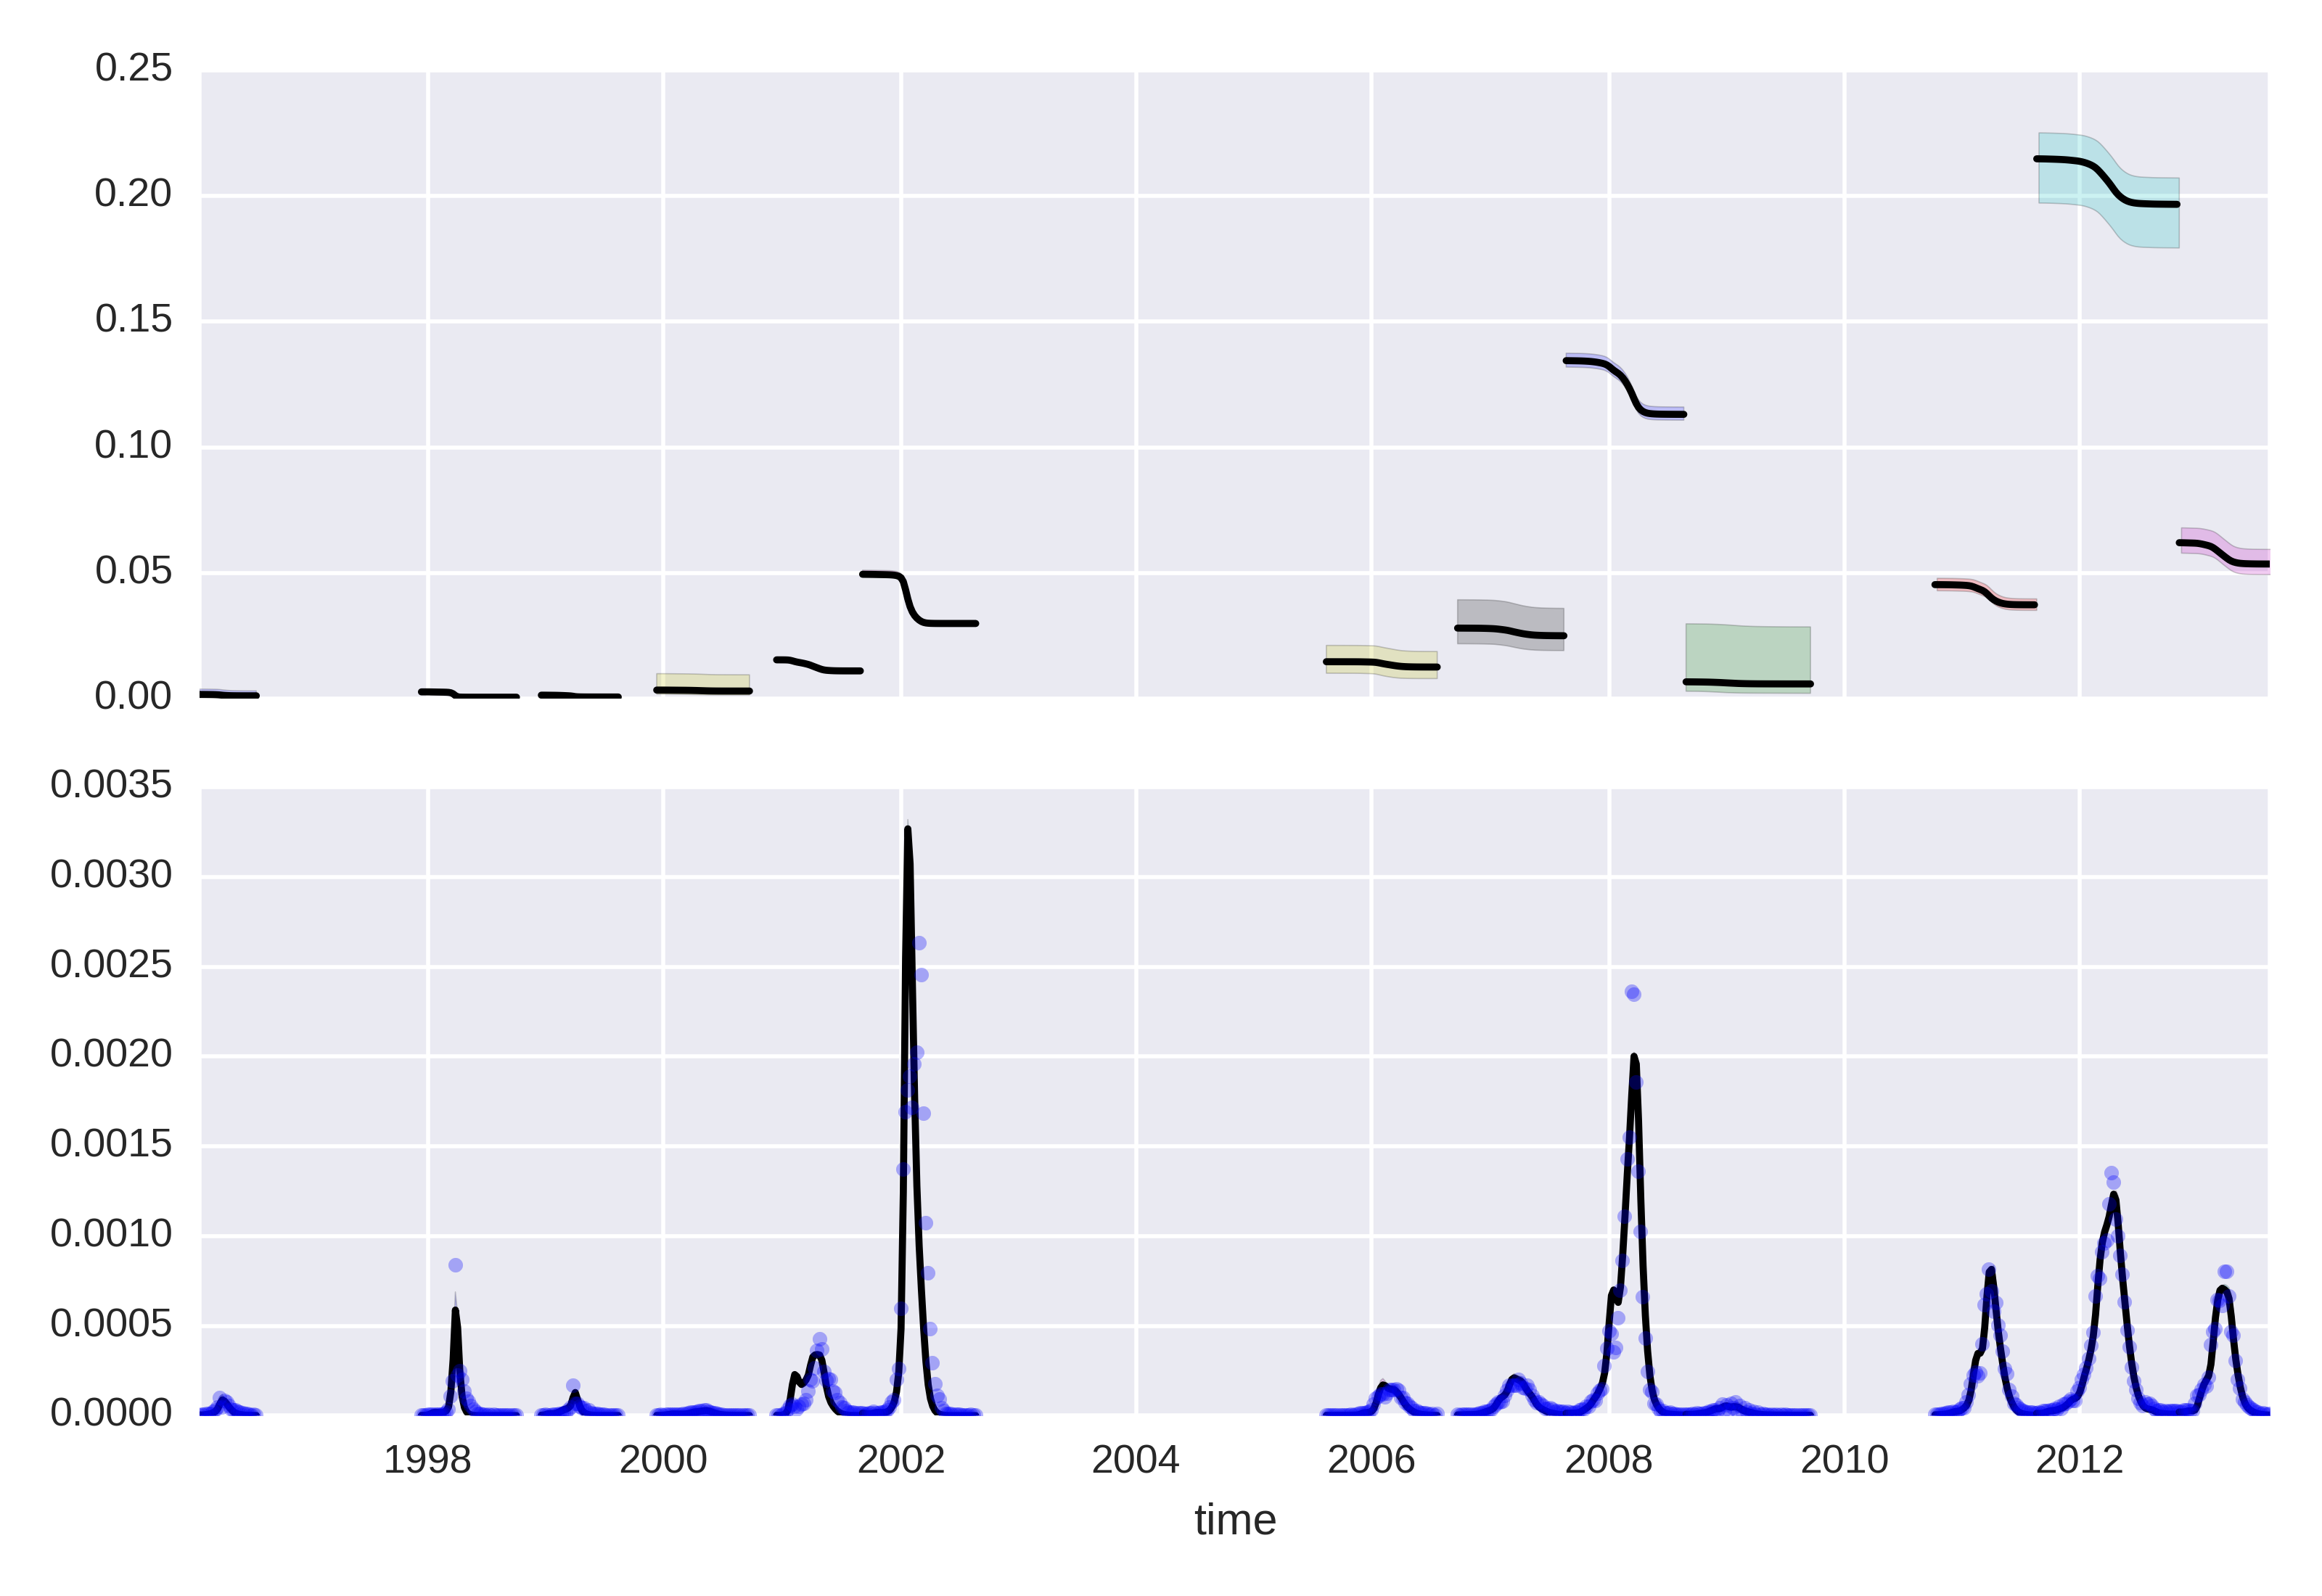
\includegraphics[width=\textwidth]{plots/concat_SI.png}
\end{center}
\caption{
{\bf Susceptibles and Infectious posterior curves.}  The curves were estimated 
only for the periods where $R_t> 1$.  The susceptible curves in the top panel 
reflect the prevalence of fraction of susceptibles to circulating strain(s) for 
each epidemic/outbreak. In the lower panel see the posterior distribution 
of infectious curves, represented by its Median and 95\% credible interval. The 
credible intervals are very narrow, and can be hard to distiguish from the 
median line. 
Scatter plot shows the observed cases. Prevalences are scaled as fractions 
of the entire population.
}
\label{Fig:S0}
\end{figure}



\section*{Tables}
% 
% See introductory notes if you wish to include sideways tables.
%
% NOTE: Please look over our table guidelines at http://www.plosone.org/static/figureGuidelines#tables to make sure that your tables meet our requirements. Certain types of spacing, cell merging, and other formatting tricks may have unintended results and will be returned for revision.
%
%\begin{table}[!ht]
%\caption{
%\bf{Table title}}
%\begin{tabular}{|c|c|c|}
%table information
%\end{tabular}
%\begin{flushleft}Table caption
%\end{flushleft}
%\label{tab:label}
% \end{table}



\begin{table}[!ht]
\caption{
\bf{Median Attack ratio and 95\% credibility intervals calculated according to 
(\ref{eq:AR2})}. $^\dag$: Year corresponds to the start of the epidemic. 
Sometimes the peak of cases occur in the following year.}
\begin{center}
\begin{tabular}{c|c|c}
\hline
Year$^\dag$ & median Attack Ratio & $S_0$ \\
\hline
1996 & 38.64\% (17.18\%-54.19\%) & 0.171\%\\
1997 & 87.31\% (73.83\%-87.31\%) & 0.273\%\\
1998 & 49.86\% (49.19\%-49.86\%) & 0.142\%\\
1999 & 10.76\% (3.72\%-20.24\%) & 0.345\%\\
2000 & 25.49\% (24.47\%-26.98\%) & 1.547\%\\
2001 & 48.12\% (46.57\%-49.15\%) & 4.951\%\\
2005 & 14.74\% (10.23\%-21.38\%) & 1.472\%\\
2006 & 11.22\% (8.00\%-14.41\%) & 2.810\%\\
2007 & 15.08\% (14.76\%-15.38\%) & 13.451\%\\
2008 & 13.73\% (3.10\%-30.84\%) & 0.672\%\\
2010 & 18.30\% (17.34\%-19.33\%) & 4.540\%\\
2011 & 8.59\% (8.20\%-9.36\%) & 21.482\%\\
2012 & 13.92\% (12.71\%-14.92\%) & 6.208\%\\

\hline
\end{tabular}


\end{center}



\label{tab:AR}
\end{table}

\section*{Supporting Information Legends}
%
% Please enter your Supporting Information captions below in the following format:
%\item{\bf Figure SX. Enter mandatory title here.} Enter optional descriptive information here.
% 
%\begin{description}
%\item {\bf}
%\item {\bf}
%\end{description}

\end{document}

